\changecolours{ScoutBlue}
\section{Gargalos do Relacional}

% -------------------------------------------------------------
% TOPICO 1 - SLIDE A: TEORIA E CUSTOS DE ESCALA
% -------------------------------------------------------------
\twocolframe[title={Escala Vertical vs. Escala Horizontal: Análise},leftcol=7cm,rightcol=7cm]{%
  \alert{Escala Vertical (Scale-Up -- RDBMS)}\par
  \itemseps[topsepi=2mm,itemsepi=3mm,labelsep=2mm,leftmargini=4mm]
  \begin{itemize}
    \item \textbf{Abordagem Clássica:} Adicionar mais CPUs, memória RAM e SSDs mais rápidos ao mesmo servidor.
    \item \textbf{Custo Exponencial:} Duplicar a capacidade pode multiplicar o preço do hardware por 10 vezes.
    \item \textbf{Teto Físico:} Limite de barramento da placa-mãe e arquitetura de processador.
    \item \textbf{Ponto Único de Falha (SPOF):} Queda da máquina derruba toda a aplicação.
  \end{itemize}
}{%
  \alert{Escala Horizontal (Scale-Out -- NoSQL)}\par
  \itemseps[topsepi=2mm,itemsepi=3mm,labelsep=2mm,leftmargini=4mm]
  \begin{itemize}
    \item \textbf{Abordagem Nativa:} Adicionar múltiplos servidores comuns em cluster (\textit{commodity hardware}).
    \item \textbf{Custo Linear:} Expansão elástica e gradual conforme a demanda real de tráfego.
    \item \textbf{Alta Resiliência:} Tolerância nativa a falhas com réplicas automáticas de dados.
    \item \textbf{Expansão Ilimitada:} Cluster cresce de 3 para centenas de nós sem interrupções.
  \end{itemize}
}

% -------------------------------------------------------------
% TOPICO 1 - SLIDE B: DIAGRAMA EM TELA CHEIA
% -------------------------------------------------------------
\begin{frame}{Topologia: Servidor Único vs. Cluster Distribuído}
  \vspace{-0.3cm}
  \makebox[\linewidth][c]{%
    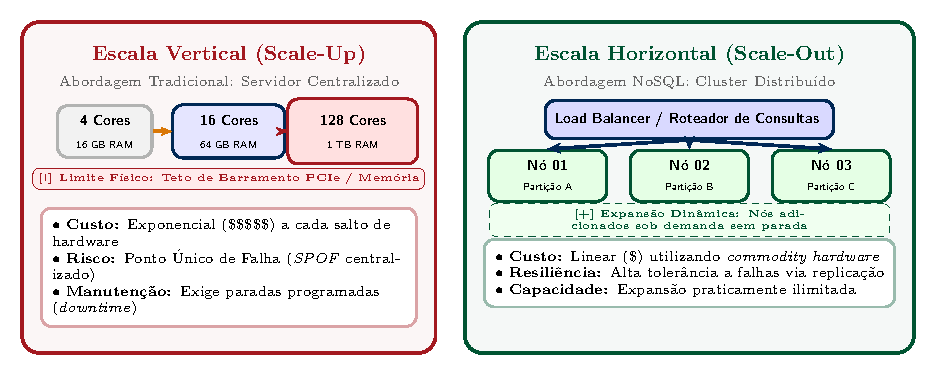
\includegraphics[width=13.2cm,height=4.8cm,keepaspectratio]{figuras/fig_escala.pdf}%
  }\par
  \vspace{0.15cm}
  \centering
  {\footnotesize \textbf{Takeaway:} \textcolor{ScoutBlue}{Enquanto o Scale-Up encontra barreiras físicas e financeiras, o Scale-Out viabiliza crescimento elástico.}}
\end{frame}

% -------------------------------------------------------------
% TOPICO 2 - SLIDE A: O PROBLEMA DOS JOINS DISTRIBUIDOS
% -------------------------------------------------------------
\twocolframe[title={O Gargalo dos JOINs em Clusters},leftcol=7cm,rightcol=7cm]{%
  \alert{Execução Local em Servidor Único}\par
  \itemseps[topsepi=2mm,itemsepi=3mm,labelsep=2mm,leftmargini=4mm]
  \begin{itemize}
    \item O motor SQL resolve o \texttt{JOIN} buscando ponteiros diretos em memória RAM ou bloco de SSD local.
    \item Operação extremamente rápida com latência inferior a 1 milissegundo.
    \item O algoritmo de junção se beneficia de índices em memória e do cache local de páginas (\textit{buffer pool}).
  \end{itemize}
}{%
  \alert{O Fenômeno do Network Shuffle}\par
  \itemseps[topsepi=2mm,itemsepi=3mm,labelsep=2mm,leftmargini=4mm]
  \begin{itemize}
    \item Em um cluster particionado, as tabelas residem em servidores físicos distintos da rede.
    \item Realizar o cruzamento obriga os nós a serializar e transmitir milhões de tuplas pelos cabos e switches.
    \item \textbf{Impacto Severo:} O tráfego massivo satura a rede e faz a latência saltar de milissegundos para dezenas de segundos!
  \end{itemize}
}

% -------------------------------------------------------------
% TOPICO 2 - SLIDE B: DIAGRAMA EM TELA CHEIA
% -------------------------------------------------------------
\begin{frame}{Anatomia do Network Shuffle: Saturação de Rede}
  \vspace{-0.3cm}
  \makebox[\linewidth][c]{%
    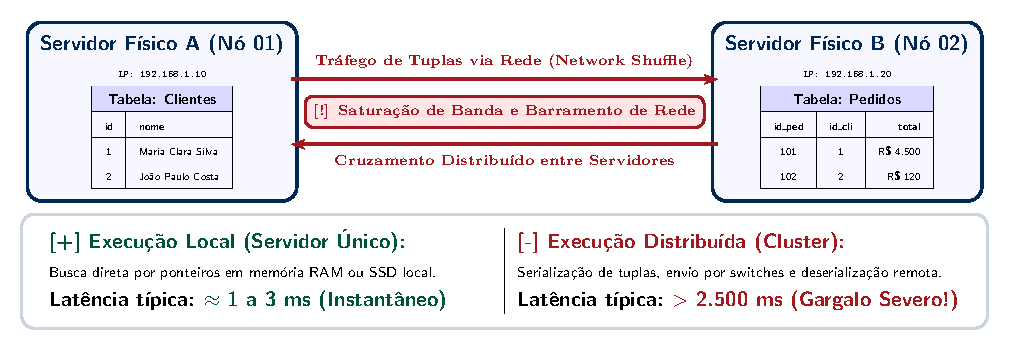
\includegraphics[width=13.2cm,height=4.8cm,keepaspectratio]{figuras/fig_gargalo_joins.pdf}%
  }\par
  \vspace{0.15cm}
  \centering
  {\footnotesize \textbf{Takeaway:} \textcolor{ScoutRed}{Cruzar dados entre servidores físicos distintos transforma a rede no gargalo principal do sistema.}}
\end{frame}

% -------------------------------------------------------------
% TOPICO 3 - SLIDE A: O DESCASAMENTO DE IMPEDANCIA
% -------------------------------------------------------------
\twocolframe[title={Descasamento de Impedância Objeto-Relacional},leftcol=7cm,rightcol=7cm]{%
  \alert{O Paradigma da Aplicação (OOP)}\par
  \itemseps[topsepi=2mm,itemsepi=3mm,labelsep=2mm,leftmargini=4mm]
  \begin{itemize}
    \item A linguagem (Python, Java) trabalha com grafos ricos de objetos em memória.
    \item Uma entidade de negócio como \texttt{Cliente} contém atributos simples, endereços aninhados e listas de pedidos.
    \item Os dados estão naturalmente agrupados para o consumo da lógica de negócio.
  \end{itemize}
}{%
  \alert{O Atrito do RDBMS \& ORM}\par
  \itemseps[topsepi=2mm,itemsepi=3mm,labelsep=2mm,leftmargini=4mm]
  \begin{itemize}
    \item A teoria relacional exige normalização estrita (3NF), forçando o fatiamento da entidade em 4 ou mais tabelas.
    \item O mapeador (ORM) adiciona sobrecarga de conversão e problemas como consultas $N+1$.
    \item \textbf{Solução em Documentos:} O formato BSON/JSON do MongoDB armazena o objeto íntegro, lido em 1 único I/O atômico!
  \end{itemize}
}

% -------------------------------------------------------------
% TOPICO 3 - SLIDE B: DIAGRAMA EM TELA CHEIA
% -------------------------------------------------------------
\begin{frame}{Mapeamento Estrutural: 3NF vs. Documento BSON Nativo}
  \vspace{-0.3cm}
  \makebox[\linewidth][c]{%
    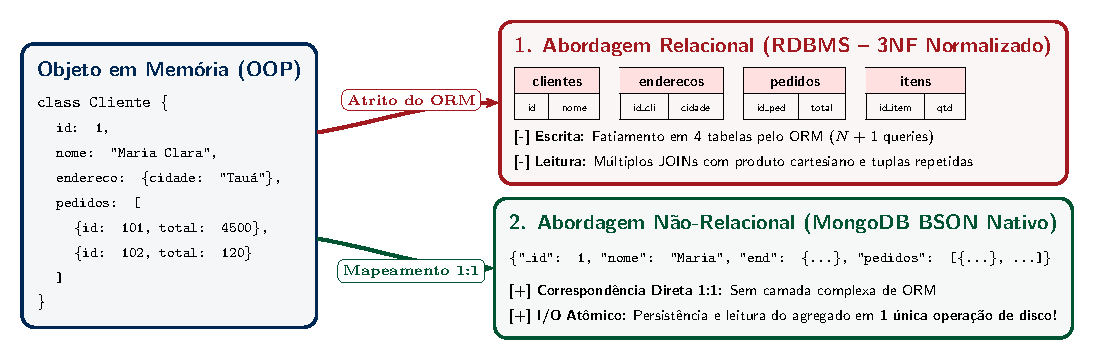
\includegraphics[width=13.2cm,height=4.8cm,keepaspectratio]{figuras/fig_impedance_mismatch.pdf}%
  }\par
  \vspace{0.15cm}
  \centering
  {\footnotesize \textbf{Takeaway:} \textcolor{ScoutGreen}{Bancos de documentos alinham a persistência física à estrutura de objetos da aplicação sem camadas de atrito.}}
\end{frame}
